\documentclass[a4paper]{llncs}
%\usepackage{fullpage}
%\usepackage{palatino}

\usepackage{makeidx}
\usepackage{amsmath}   
\usepackage[retainorgcmds]{IEEEtrantools}
\usepackage{thumbpdf}
\usepackage{multicol}   
\usepackage{graphicx}   
\usepackage{listings}
\usepackage{algorithm}
\usepackage{algorithmic}
\usepackage{tikz}
\usepackage{subfigure}

\usepackage[
  pagebackref,
  pdfpagelabels,
  extension=pdf,
]{hyperref}
\hypersetup{ 
  pdftitle          = {Is Learning Small World?},
  pdfsubject        = {Is Learning Small World?},
  pdfauthor         = {Arun Tejasvi Chaganty, Prateek Gaur},
  pdfkeywords       = {},
  pdfcreator        = {pdflatex},
  pdfproducer       = {LaTeX with hyperref and thumbpdf},
  pdfstartpage      = {1},
  pdfpagemode       = UseThumbs,
  colorlinks        = true,
  linkcolor         = red,
  anchorcolor       = red,
  citecolor         = blue,
  filecolor         = red,
  urlcolor          = red
}

% Section References
\newcommand{\secref}[1] {\hyperref[#1]{Section~\ref*{#1}}}
\newcommand{\eqnref}[1] {Equation \eqref{#1}}
\newcommand{\thmref}[1] {Theorem \ref{#1}}
\newcommand{\lmref}[1] {Lemma \ref{#1}}
\newcommand{\algoref}[1] {\hyperref[#1]{Algorithm~\ref*{#1}}}
%\renewcommand{\algorithmiccomment}[1]{\textit{// #1}}
%\theoremstyle{plain} \newtheorem{thm}{Theorem}

%Math Operators
\DeclareMathOperator {\argmax} {argmax}
\DeclareMathOperator {\sgn} {sgn}
\DeclareMathOperator {\trace} {tr}
\DeclareMathOperator{\E} {E}
\DeclareMathOperator{\Var} {Var}

\renewcommand{\Re} {\mathbb{R}}

\newcommand{\ud}{\, \mathrm{d}}
\newcommand{\diff}[1] {\frac{\partial}{\, \partial #1}}
\newcommand{\diffn}[2] {\frac{\partial^{#2}}{\, \partial {#1}^{#2}}}
\newcommand{\tuple}[1] {\langle #1 \rangle}

%Short hand
\newcommand{\mdp} {\ensuremath{\mathcal{M}}}
\newcommand{\states} {\mathcal{S}}
\newcommand{\actions} {\mathcal{A}}
\newcommand{\transitions} {\mathcal{P}}
\newcommand{\rewards} {\mathcal{R}}
\newcommand{\graph} {\mathcal{G}}
\newcommand{\policy} {\pi}
\newcommand{\initset} {\mathcal{I}}
\newcommand{\stopcond} {\beta}
\newcommand{\option} {\tuple{ \initset,\policy,\stopcond} }
\newcommand{\options} {\mathcal{O}}

%Math Operators
\DeclareMathOperator {\ball} {B}
\DeclareMathOperator {\ballf} {B^{f}}
\DeclareMathOperator {\sball} {b}
\DeclareMathOperator {\sballf} {b^{f}}

%Short hand
\newcommand{\arbcnst} {\tilde{c}}
\newcommand{\greedyalgo} {\ensuremath{\mathcal{GA}~}}


\title{Is Learning Small World?}
\author{ Arun Tejasvi Chaganty \inst{1} \and Prateek Gaur \inst{1} } 
\institute{ Department of Computer Science and Engineering, \\
            IIT Madras, Chennai, India - 600036 }

\pagestyle{headings}  % switches on printing of running heads

\frontmatter
\mainmatter

\begin{document}

\maketitle
%\pagebreak

% Outline
\begin{abstract}

Understanding how we are able to perform a diverse set of complex tasks
has been a central question for the Artificial Intelligence community.
One popular approach is to use temporal abstraction as a framework to
capture the notion of subtasks. However, this transfers the problem to
finding the right subtasks, which is still an open problem. Existing
approaches for subtask generation require too much knowledge of the
environment, and the abstractions they create can overwhelm the agent.
We propose a simple algorithm inspired by small world networks to learn
subtasks while solving a task that requires virtually no information of
the environment. Additionally, we show that the subtasks we learn can be
easily composed by the agent to solve any other task; more formally, we
prove that any task can be solved using only a logarithmic combination
of these subtasks and primitive actions. Experimental results show that
the subtasks we generate outperform other popular subtask generation
schemes on standard domains. 

%\draft{What is our contribution?}
% Relevance to lifelong learning?

\end{abstract}

\section{Introduction}
\label{sec:intro}

% General Introduction
In large domains, RL agents generally require a large number of samples to learn
a good policy. The options framework proposed by Sutton, Precup and Singh
\cite{SuttonPrecupSingh1998} provides extended actions for which a policy is
already learnt, reducing the complexity of the learning task, and generally
making the learning task faster.  An open question in the options framework is
discovering the options themselves.  There has been substantial work to learn
options, mainly focussed around identifying ``bottleneck'' states, either
empirically as in the work bye Stolle \cite{Stolle}, or more recently, using
graph theoretic methods like betweeness \cite{Simsek} or graph partitions
\cite{Simsek2005} explored by Simsek and Barto.

% Motivation
In this work, we propose a method for creating options motivated from a
cognitive perspective, based on the following hypothesis: we memorise many
actions, not necessarily bottleneck ones, and evolve them. Based on their
necessity in solving problems these actions are either reinforced, or gradually
forgotten. The actions could be of varying complexity, and it is intuitive to
expect that we probably learn a great deal more {\em simple} actions than
complex ones. In context of the options framework, these actions correspond to
options, and ``complex actions'' correspond to longer options.

% Our options
A desirable set of options gives the agent a set of skills which can be put
together to efficiently accomplish almost any task. From the perspective of the
state-space interaction graph, this is similar to the problem of distributed
search studied by Kleinberg \cite{Kleinberg}; adding edges to a graph such that
any node can be efficiently reached. Guided by this intuition, the method we
propose generates options using a generalisation of the inverse-square law,
along the lines of the small-world graph generation model proposed by Kleinberg.

% Summary of the results
Our results show that agents trained using our `small-world' options indeed
perform well, and converge to optimal performance quickly and with little
variance. 


\section{Approach}
\label{sec:approach}

% MDPs
Before we describe our approach for generating options, we briefly review Markov
Decision Processes (MDPs) and options framework. An MDP $\tuple{
    \states,\actions,\rewards }$ is a standard representation for a RL problem,
where $\states$ is the set of states in the world, $\actions$ is the set of
actions that take the agent from one state to another with some transition
probability, and $rewards$ is the set of rewards obtained when moving from one
state to another. The objective is to find a decision procedure or policy $\pi$
that maximises the return, or the rewards accumulated in the long run. 

% Options
An option $\option$ is described by an initiation set $\initset \subset
\states$, a policy $\pi$, and a terminating condition $\beta$. An agent can
exercise an option in any state $s \in \initset$, following which, it will
follow the policy $\pi$ described by the option, until the terminating condition
$\beta(s)$ is satisfied. The terminating condition $\beta$ can be stochastic as
well. 

% Example

\begin{figure}[h]
    \center
    \documentclass{article}
\usepackage{standalone}
\usepackage{tikz}
\usetikzlibrary{external}
\tikzexternalize % activate!

\begin{document}
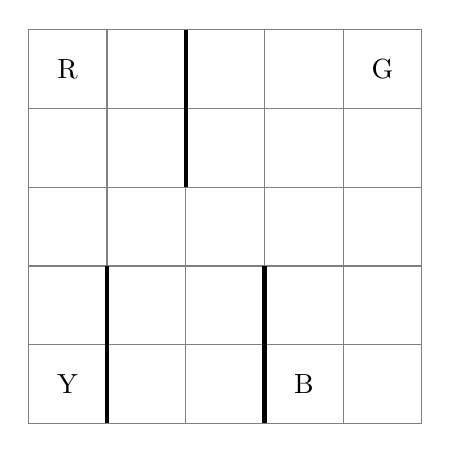
\begin{tikzpicture}
    % Grid
    \draw[step=1,color=gray] (0,0) grid (5,5);
    
    % Walls
    \draw[line width=1.5pt] (2,5) -- (2,3);
    \draw[line width=1.5pt] (1,0) -- (1,2);
    \draw[line width=1.5pt] (3,0) -- (3,2);

    % Pads
    \draw (0.5,4.5) node {R};
    \draw (0.5,0.5) node {Y};
    \draw (3.5,0.5) node {B};
    \draw (4.5,4.5) node {G};
\end{tikzpicture}
\end{document}

    \caption{The Taxi Domain}
    \label{fig:taxi-domain}
\end{figure}

To make the discussion more tangible, let us look at an example, the Taxi
domain, shown in \autoref{fig:taxi-domain}. The agent is a taxi navigating in
this road-map. It must pick up a passenger at one of the 4 pads, A, B, C or D.
Subsequently, it must carry the passenger to a destination, which is also one of
the above four pads. The states of the taxi would then be the location of the
passenger (in one of the four pads, or within the taxi), the destination of the
passenger, and location of the taxi in the map. The actions the taxi can perform
are moving up, down, left or right in the map, as well as pick up a passenger or
drop him at the destination.  Typical options for such a domain would be an
option that can be started anywhere, and has a policy that takes the taxi to the
one of the pads in the shortest possible manner. Such an option is generic, and
does not depend on where the passenger or destination are. The RL agent must
then learn to choose the right option when picking up the passenger.

\begin{figure}[h]
    \center
    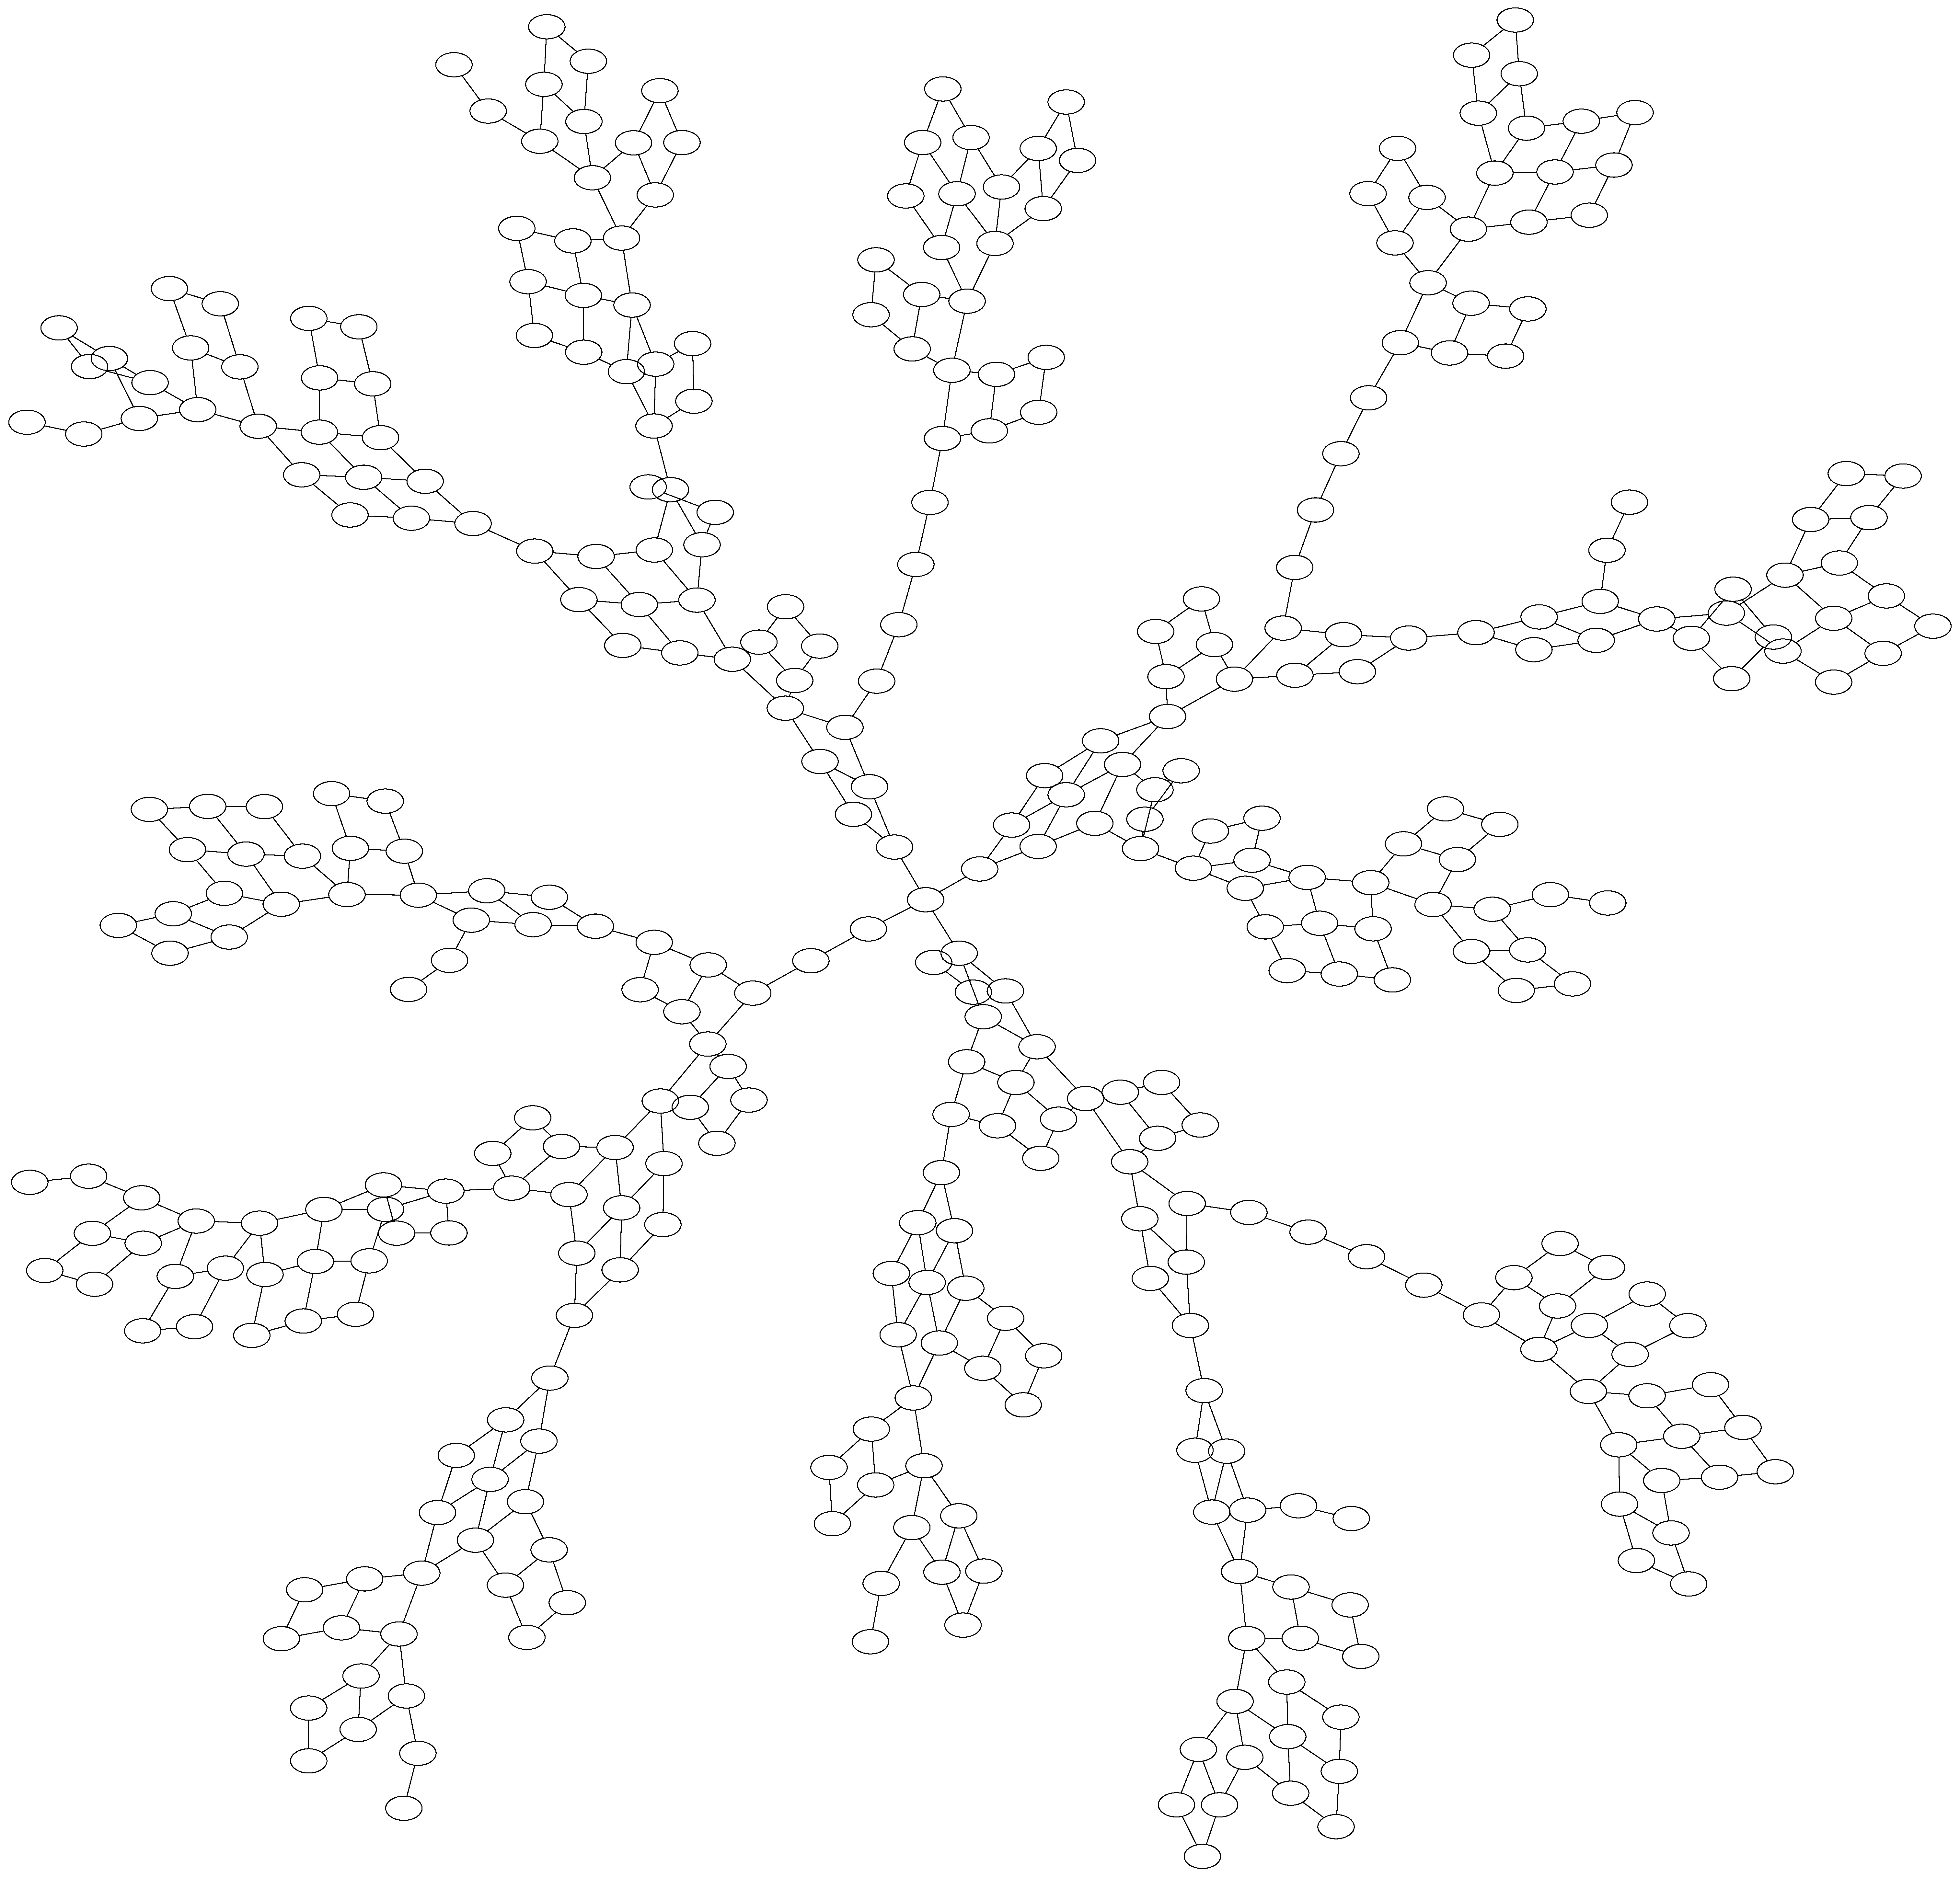
\includegraphics[width=3in]{figures/taxi1}
    \caption{State Space Graph for the Taxi Domain}
    \label{fig:taxi-graph}
\end{figure}

% Graph-based
It is easy to construct a graph $\graph$ out of the state-space described by an
MDP. The states $\states$ become the nodes of the graph, and $\actions$ become
the edges, with the transition probabilites serving as the weights. The edges
are also attributed with the rewards described by $\rewards$. Options can be
viewed to be paths along the graph. The Taxi domain just defined translates to
a graph shown in \autoref{fig:taxi-graph}.

% Constructing Options 
We construct an option `short-circuiting' two states using a policy constructed
from the shortest path on this graph. For every state $x$, we select a state to
be short-circuited $y$ with using a multinomial distribution with weight
proportional to the distance between them in the state space, i.e. $w(x,y)
    \propto d(x,y)^{-r}$. 

Another example of constructing an option on this graph would be to define a
policy that takes any state to a particular one along the shortest path. This is
the approach adopted by Simsek and Barto in \cite{Simsek}, where local maxima of
the betweenness scores are used to identify bottlenecks, and options defined to
reach these bottlenecks optimally from any state.

% Describe Macro-Q and Intra-Option-Q
Several learning algorithms have been proposed for agents using options
\cite{SuttonPrecupSingh1998,BartoMahadevan}. A simple such method is Macro
Q-learning, a generalisation of the Q-learning methods. The MacroQ algorithm
updates the value function only after completion of the option. If the option
$o$ was initiated in the state $s$, and continue for $k$ steps before
terminating in $s'$, the corresponding back-up will be,

\begin{IEEEeqnarray*}{rCl}
    Q(s,o) &=& Q(s,o) + \alpha [ r + \gamma^{k} \max_{o' \in \options_{s'} \cup \actions_{s'}} Q(s',o') - Q(s,o) ].
\end{IEEEeqnarray*}

Another method, Intra-option Q-learning, exploits the experience gathered during
the trajectory, instead of only at the end of it. In this approach, every step
from $s$ to $s'$ using $a \in \actions$ is used to back up the value function of
every option $o \in \options$ which can be used in $s$, and whose policy has a
non-zero probability of using the action $a$ using the following update,

\begin{IEEEeqnarray*}{rCl}
    Q(s,o) &=& Q(s,o) + \alpha [ r + \gamma Q(s',o) - Q(s,o) ].
\end{IEEEeqnarray*}
\noindent
The value-function for every action along the trajectory is also updated, using
the usual Q-learning backups.

% \begin{IEEEeqnarray*}{rCl}
%     x &=& y \\
%       &=& z \\
% \end{IEEEeqnarray*}

% \begin{figure}[s]
%     \centering
%     \includegraphics[width=5in]{filename}
%     \caption{ }
%     \label{fig:high-variance-rtt}
% \end{figure}

%\section{Empirical Performance}
\label{sec:experiments}
% Experimental results

% Graphs
\begin{figure}[h]
\centering
\subfigure[$P_2$-Distributed Options]{
\includegraphics[height=2in]{figures/rooms-options}
\label{fig:rooms-options}
}
\subfigure[Cumulative Return]{
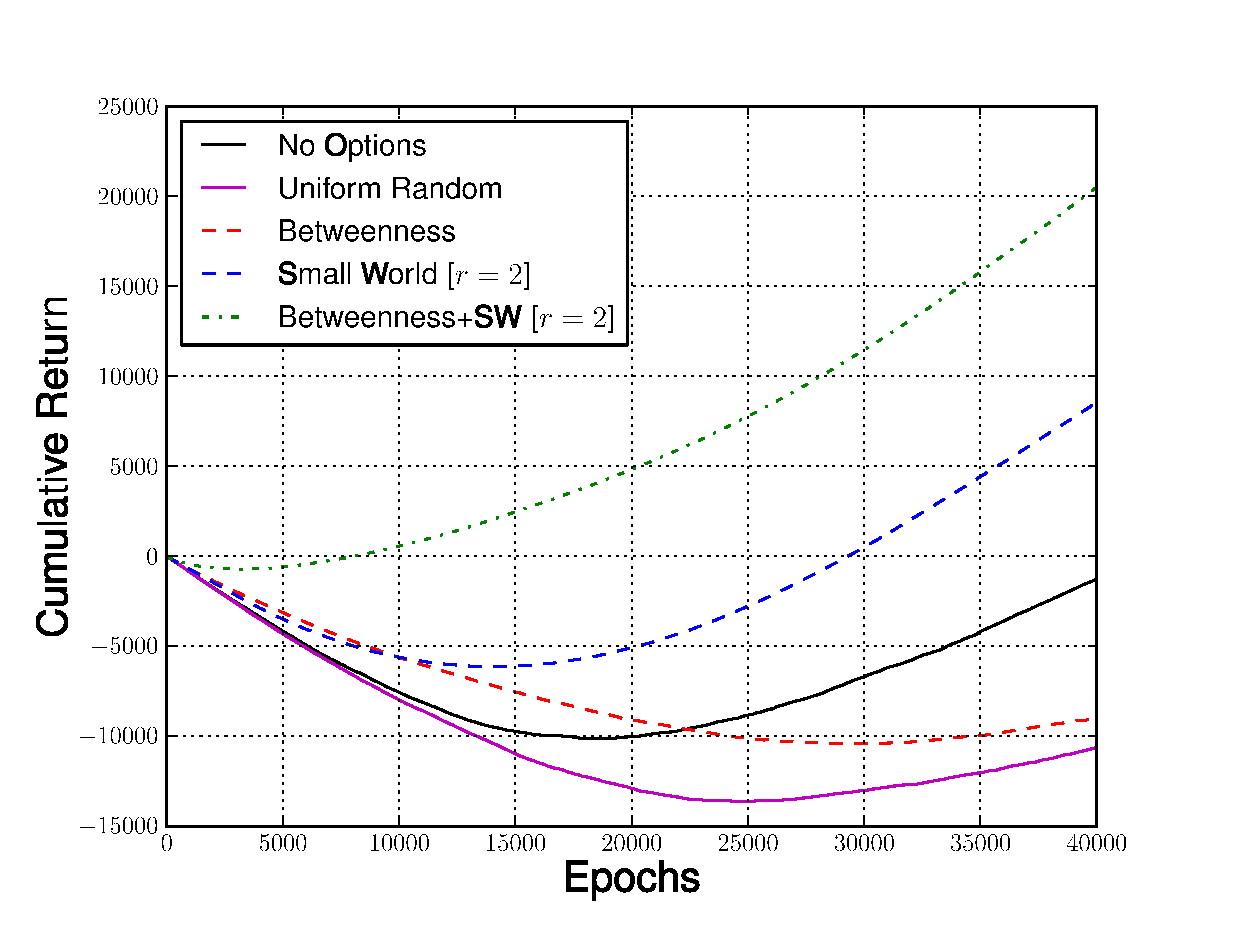
\includegraphics[height=2.2in]{figures/rooms-algos-200}
\label{fig:rooms-performance}
}
\label{fig:rooms}
\caption{Results on the Rooms Domain}
\end{figure}

% Brief description of Rooms, Taxi and Arbitrary Navigation domains.
We trained agents using the MacroQ algorithm, and tested it on three
standard domains, Taxi, Rooms and a $20\times20$ arbitrary navigation
task, and compared the performance of agents using options generated
(i) using betweenness centrality, (ii) using $P_0$ (uniformly random
paths), (iii) using paths between nodes selected using $P_{r>0}$, and
(iv) using a combination of (i) and (iii).  The performance of
$P_r$-distributed options was worst when $r=0$, and increased to peak
at a particular $r$ before decreasing again; behaviour also observed
in Kleinberg's work. With appropriate $r$, $P_r$-distributed options
accumulate significant return, and outperform bottleneck-based methods
on navigation tasks. 

% Observations
% When goal state and start state are further apart, the options that stand out
% are more


\section{Conclusions and Future Work}
\label{sec:conclusions}

% Contributions
% - new scheme for generating options
We have devised a new scheme to generate options based on small world
network model. The options generated satisfy an intuitive criteria, that
the subtasks learnt should be easily composed to solve any other task.
The options greatly improve the connectivity properties of the domain,
without leading to a state space blow up. Finally, they are interesting
from a theoretical perspective, as they require only a logarithmic
number of decisions required in a learning task.

% - absolutely model-free
Experiments run on standard domains show significantly faster learning
rates using small world options. At the same time, we have shown that
learning small world options can be cheaper than learning bottleneck
options, using a natural algorithm that extracts options from a handful
of tasks it has solved. Another advantage of the scheme is that is does
not require a model of the MDP. 

% Further work
% - dynamically add/remove options
% - figuring out r
As future work, we would like to characterise what the exponent $r$
should be in a general domain. Given the ease with which options can be
discovered, it would be interesting to experiment with a dynamic scheme
that adds options on the fly, while solving tasks.



\bibliographystyle{alpha}
\bibliography{library}{}

%\newpage
%\appendix

%
\section{Code}
\label{sec:code}
% \lstset{language=TCL, basicstyle=\small, showstringspaces=false, numbers=left, numberstyle=\tiny }
% \lstinputlisting{many2one.tcl}


\end{document}

